\documentclass[11pt, oneside]{article} 
\usepackage{geometry}
\geometry{letterpaper} 
\usepackage{graphicx}
	
\usepackage{amssymb}
\usepackage{amsmath}
\usepackage{parskip}
\usepackage{color}
\usepackage{hyperref}

\graphicspath{{/Users/telliott_admin/Dropbox/Tex/png/}}
% \begin{center} 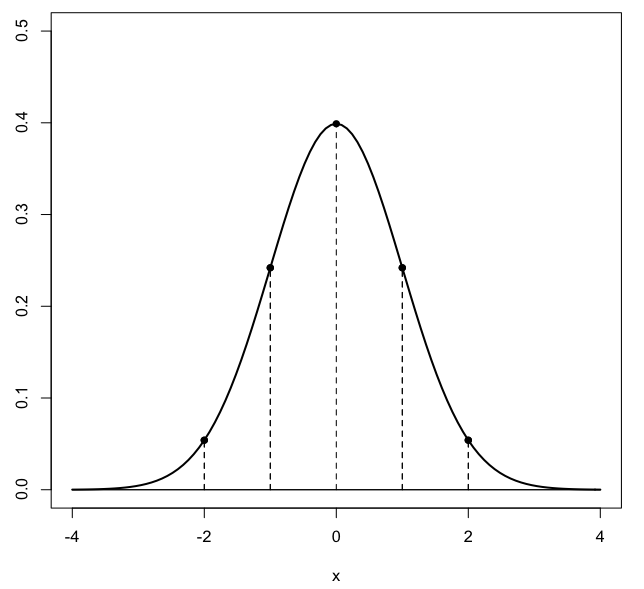
\includegraphics [scale=0.4] {gauss3.png} \end{center}

\title{Circular orbits}
\date{}

\begin{document}
\maketitle
\Large

This part of the book is focused on geometry, and we take a look at Eratosthenes in this chapter as an important Greek scholar.

The widely held theory, that the ancient world believed the earth to be flat, is just wrong.  People with any level of sophistication not only knew the earth is roughly spherical but also knew its size within a few percent of the true value.

One likely basis is the false story that Columbus had trouble getting financing for his proposed trip to China because everyone thought he would fall off the edge of the earth.  This was a tall tale invented by Washington Irving, who also made up several remarkable fables about George Washington.

The real reason the Italians and the Portuguese thought Columbus would fail is that they had a pretty good idea of the size of the spherical earth and thus of the distance to China, while the over-optimistic Columbus believed it was about half the true value.  The prospective financiers knew that he was not able to carry the supplies necessary for a trip of this length.

Morris Kline (\emph{Mathematics and the Physical World}) says that the error is due to geographers after Eratosthenes, who reduced the estimated circumference from 24,000 to 17,000 miles.

\subsection*{Eratosthenes}

Views of the Greek philosophers on the earth and its sphericity are detailed here

\url{https://www.iep.utm.edu/thales/#SH8d}

Here is a partial quotation:

\begin{quote}
There are several good reasons to accept that Thales envisaged the earth as spherical. Aristotle used these arguments to support his own view [...] . First is the fact that during a solar eclipse, the shadow caused by the interposition of the earth between the sun and the moon is always convex; therefore the earth must be spherical. In other words, if the earth were a flat disk, the shadow cast during an eclipse would be elliptical. Second, Thales, who is acknowledged as an observer of the heavens, would have observed that stars which are visible in a certain locality may not be visible further to the north or south, a phenomen[on] which could be explained within the understanding of a spherical earth.
\end{quote}

\url{https://en.wikipedia.org/wiki/Eratosthenes}

Eratosthenes (ca. 276 - 195 BCE) measured the circumference of the earth from this observation:  at high noon on June 21st there was no shadow  seen at Syene, e.g., allegedly from a stick in the ground.  Some people say it was a deep well, where the bottom was illuminated at midday.

Syene is presently known as Aswan.  It is on the Nile about 150 miles upstream of Luxor, which includes the famous site called the Valley of the Kings.  At 24.1 degrees north latitude, Aswan or Syene is close enough to having the sun directly overhead on June 21.  (The "Tropic of Cancer" is at 23 degrees, 26 minutes north).

\begin{center} 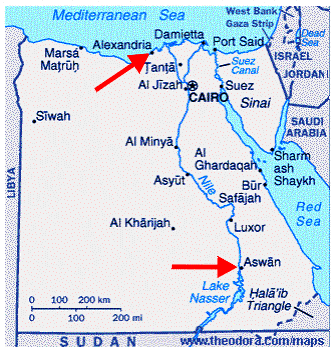
\includegraphics [scale=0.6] {aswan.png} \end{center}

This news about the lack of a shadow at Syene reached Alexandria, a famous center of learning of the ancient world.  Alexandria lies on the Mediterranean some 500 miles north of Syene, and anyone there who was looking could observe that at high noon on June 21st there \emph{was a shadow}.  This shadow Eratosthenes measured to be some 7 degrees and a bit (7 degrees and 10 minutes).

\begin{center} 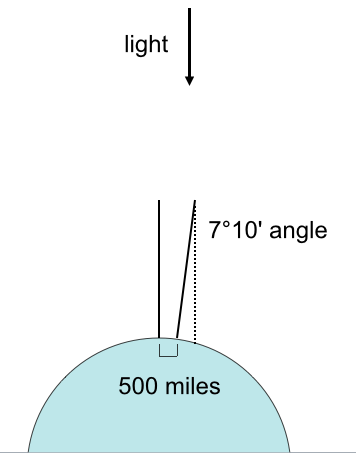
\includegraphics [scale=0.4] {eratosthenes.png} \end{center}

A full 360 degrees divided by 7 degrees and a bit is approximately 50.  So we can calculate on this basis that the circumference of the earth is about $50 \times 500 = 25000$ miles.  That's pretty close to the correct value.

For this calculation, we assume that the sun's rays are effectively parallel (not a bad assumption given a distance of 93 million miles).  Then we just use this:

\begin{center} 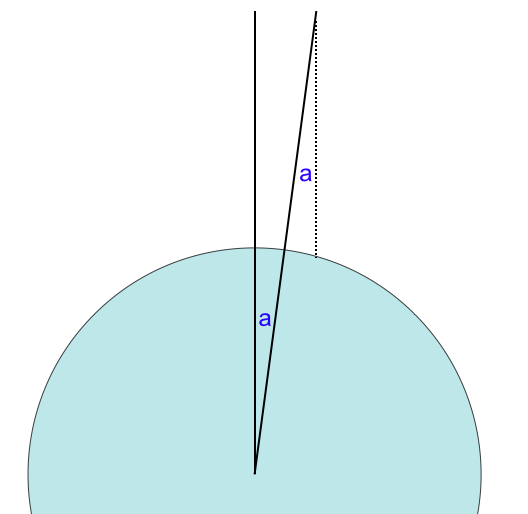
\includegraphics [scale=0.3] {eratosthenes2.png} \end{center} 

an application of the alternate-interior-angles theorem.

It is curious how the distance from Alexandria to Syene was calculated [Kline]. "Camel trains, which usually traveled 100 stadia a day, took 50 days to reach Syene.  Hence the distance was 5000 stadia...It is believed that a stadium was 157 meters."  We obtain
\[ 157 \times 5000 \times 50 = 39,250 \ \text{km} \]
That's a much better estimate than a method that relies on camels really deserves.

\subsection*{The sieve of Eratosthenes}

Eratosthenes is famous in mathematics for his "sieve" which allows one to compute the prime numbers in an economical fashion.  This next section really has nothing to do with calculus, but it is inspired mathematics.

The sieve is operated by first enumerating all the integers to some upper limit (here $120$).  To do things manually it is convenient to use rows with $10$ values, so there are $12$ of them in all.  Most of the boxes have not yet been numbered.

Starting with the first prime number, $2$ (red), eliminate all the numbers divisible by $2$ (all the even numbers).  Here this has been done by coloring red all of the squares in the even numbered columns (all numbers ending in $2,4,6,8,0$).

\begin{center} 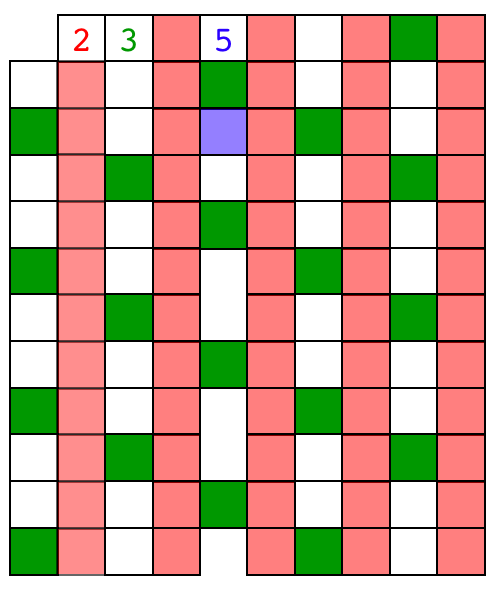
\includegraphics [scale=0.35] {sieve6.png} \end{center} 

Next, do the same thing with $3$ (green).  $6$ was already eliminated previously, but all odd multiples of $3$ like $9$ and $15$ go away at this step.

The next larger number that still has a white square is $5$.  The only squares eliminated are the white ones in the fifth row. The first value specifically eliminated at the $5$ step is $25$.  Continue with $7$, eliminating $49, 77, 91$ and $119$.

\begin{center} 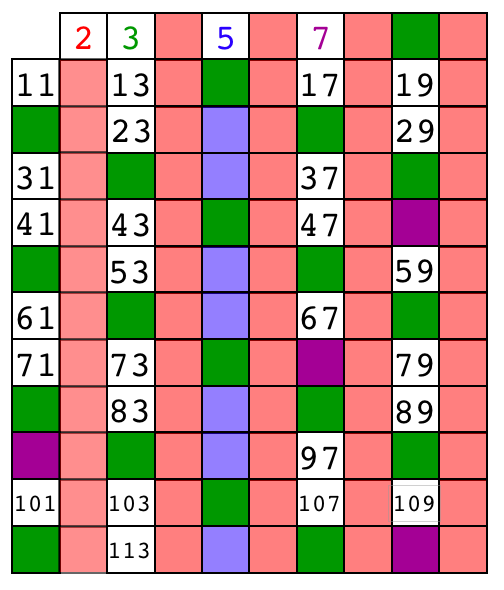
\includegraphics [scale=0.35] {sieve7.png} \end{center} 

The sieve ends when the number for the beginning of the next round, the smallest number not yet eliminated, is greater than the square root of the upper limit (here $\sqrt{120}$).  So $7$ is used for the last round, because after that round the smallest remaining integer is $11$, but we terminate since $11^2 > 120$.

The graphic shows all the numbers which have yet to be eliminated after the round of $7$.   All of these numbers, $11$, $13$, $17$, and so on, as well as those used as divisors for each round of the sieve ($2, 3, 5, 7$), are prime numbers.

By testing for division by $2, 3, 5$ and $7$, we have found the first $30$ prime numbers.

From a performance standpoint, it is important that we do not need to carry out division.  All that is really needed is repeated addition.  Coding this algorithm in, say, Python is a good challenge.  A bigger challenge is to come up with a method to \emph{grow} the list of primes on demand.  This can be done by keeping track of the first value to be tested above the limit, for each prime in the current list.

\subsection*{Aristarchus}

Aristarchus of Samos (310-230 BCE) wrote a famous book in which he calculated the relative sizes of the sun and the moon and their distances from earth.

One straightforward observation is that the apparent size of the sun and moon in the sky is about the same.  This can be seen during a solar eclipse, or observed at any other time by holding a disk up at a fixed distance from the eye, (while taking care to block most of the sun's rays).  The value is approximately one-half degree.

Since the distance to the sun is much greater than that to the moon (see below), we can infer that the sun is much larger than the moon.

The central idea of Aristarchus is that, at half moon, the geometry of the three orbs is like this:

\begin{center} 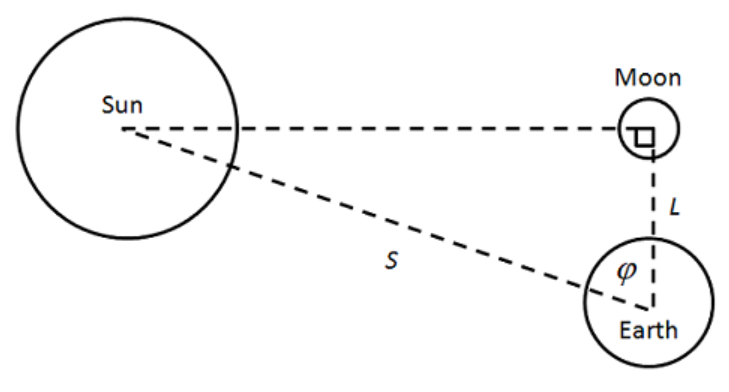
\includegraphics [scale=0.4] {half_moon.png} \end{center}

In other words, when the phase is half moon and that moon is exactly overhead, the sun has not yet set, but is a bit above the horizon. 

If $S$ is the distance to the sun and $L$ is that to the moon, he estimated that

\[ 18 < \frac{S}{L} < 20 \]

with the same ratio for their sizes.  Unfortunately, this is not a particularly good estimate.  The true value is about 390.  Aristarchus obtained a value of 20 for the Earth-Moon distance in Earth radii.  The correct value is about 60.  Much better estimates were obtained later, by Hipparchus and Ptolemy.

However, Aristarchus made up for this by being the first person to propose a heliocentric theory of the solar system:  that the earth and planets rotate around the sun.

\url{https://en.wikipedia.org/wiki/On_the_Sizes_and_Distances_(Aristarchus)}

\subsection*{quick estimate}

Here is an estimate for the earth-moon distance based on a lunar eclipse.

One measures the time it takes for a complete, total eclipse.  From the first shadow of the earth on the moon to the last, that time is about 3 hr.  The moon has moved approximately 1 earth diameter in its orbit in that time.

However, we must correct for the fact that the first and last shadows occur on opposite edges of the moon.  It was noted that the shape of the eclipse suggests the earth's diameter (at that distance) is about 2.5 moon diameters.  So the moon has actually moved (2.5 + 1.0)/2.5 = 1.4 earth diameters in the given time.  The relevant time becomes 2.14 hr.

Any correction for the true size of the earth's diameter is minimal because the earth-moon system is so far from the source of illumination.

The other piece of information we need is the time for a full revolution, one lunar cycle.  This part is tricky.  Naively, you'd look for the moon to be in the same place against the fixed stars (27 days, c. 8 hr).  This is off because the earth has moved in the meantime --- there is a parallax error.  As a rough correction, mutliply by 360/330 degrees.  The result in hours is 715.

The circumference of the orbit is then

\[ 715 / 2.143 = 333 \]
earth diameters.

This gives a radius of 53 earth diameters, which is not too far from 60.


\end{document}